\documentclass[11pt]{article} % use larger type; default would be 10pt
\usepackage[utf8]{inputenc} % set input encoding (not needed with XeLaTeX)
\usepackage{fullpage}
\usepackage{graphicx} % support the \includegraphics command and options
\usepackage{caption}
\usepackage{subcaption}
\usepackage{amsmath}
\usepackage{amssymb}
\newcommand{\drv}[2]{\ensuremath{\frac{d #1}{d #2}}}
\newcommand{\ddrv}[2]{\ensuremath{\frac{d^2 #1}{d^2 #2}}}
\newcommand{\into}{\ensuremath{\int_{-1}^1}}
\newcommand{\intz}{\ensuremath{\int_0^1}}
\newcommand{\intf}{\ensuremath{\int_{-\infty}^\infty}}
\newcommand{\inti}{\ensuremath{\int_{x_{i-1/2}}^{x_{i+1/2}}}}
\newcommand{\intO}{\ensuremath{\int_{4\pi}}}
\newcommand{\order}[1]{\ensuremath{\mathcal{O}(#1)}}
\newcommand{\He}{\ensuremath{\mbox{He}}}
\newcommand{\expv}[1]{\ensuremath{\langle #1 \rangle}}

\title{1D problem testing}
\author{Paul Talbot}
%\date{}

\begin{document}
\maketitle

Equation to solve:
\begin{equation}
-\nabla D_g\nabla\phi_g+\sigma_{a,g}\phi_g=\sum_{g'}\sigma_s^{g'g}\phi_{g'}+\frac{\chi_g}{k}\sum_{g'}\nu\sigma_{f,g'}\phi_{g'}, \hspace{15pt}g\in(1,2),
\end{equation}

The problem is 2D, but we simulate 1D by imposing reflecting boundaries on the top and bottom of the problem.  The physical mesh is four-by-four regions, but each region consists of an identical material with properties described in Table \ref{matprops}.  The flux profiles for either group are shown in Fig. \ref{fluxes}.  Note that the axes label numeric cells, not centimeters; each cell is 2 cm square.
\begin{table}
\begin{center}
\begin{tabular}{c|l l}
Property & Group 1 & Group 2 \\ \hline
$D$ & 1.255 & 0.211\\
$\Sigma_a$ & 0.008252 & 0.09434\\
$\nu\Sigma_f$ & 0.004602 & 0.1091\\
$\Sigma^{1\to2}_s$ & 0.02533 & 0\\
$\chi$ & 1 & 0\\
\end{tabular}
\caption{Material properties}
\label{matprops}
\end{center}
\end{table}

\begin{figure}[h!]
\centering
  \begin{subfigure}[b]{0.45 \textwidth}
   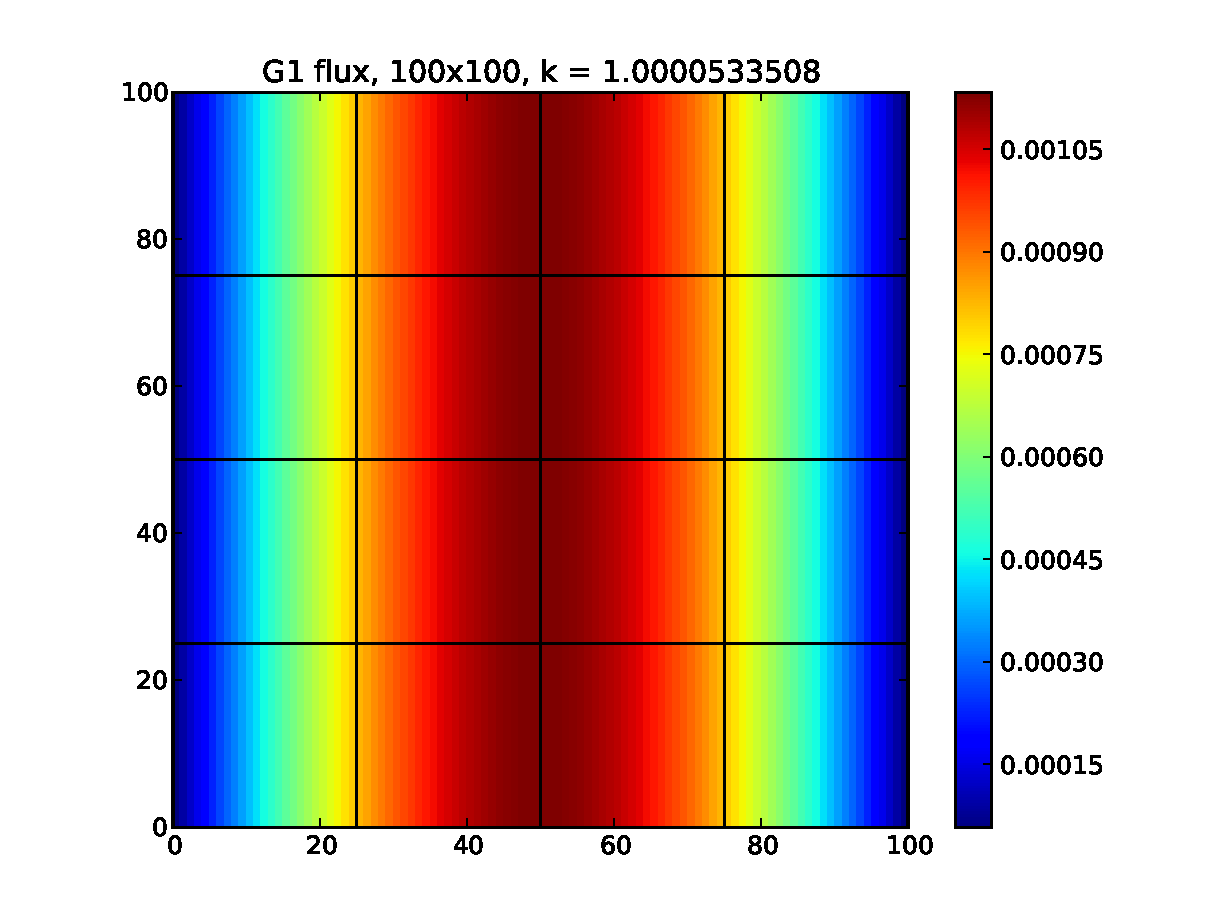
\includegraphics[width=\textwidth]{g1_50_flux}
   \caption{High-energy flux}
  \end{subfigure}
  \begin{subfigure}[b]{0.45\textwidth}
   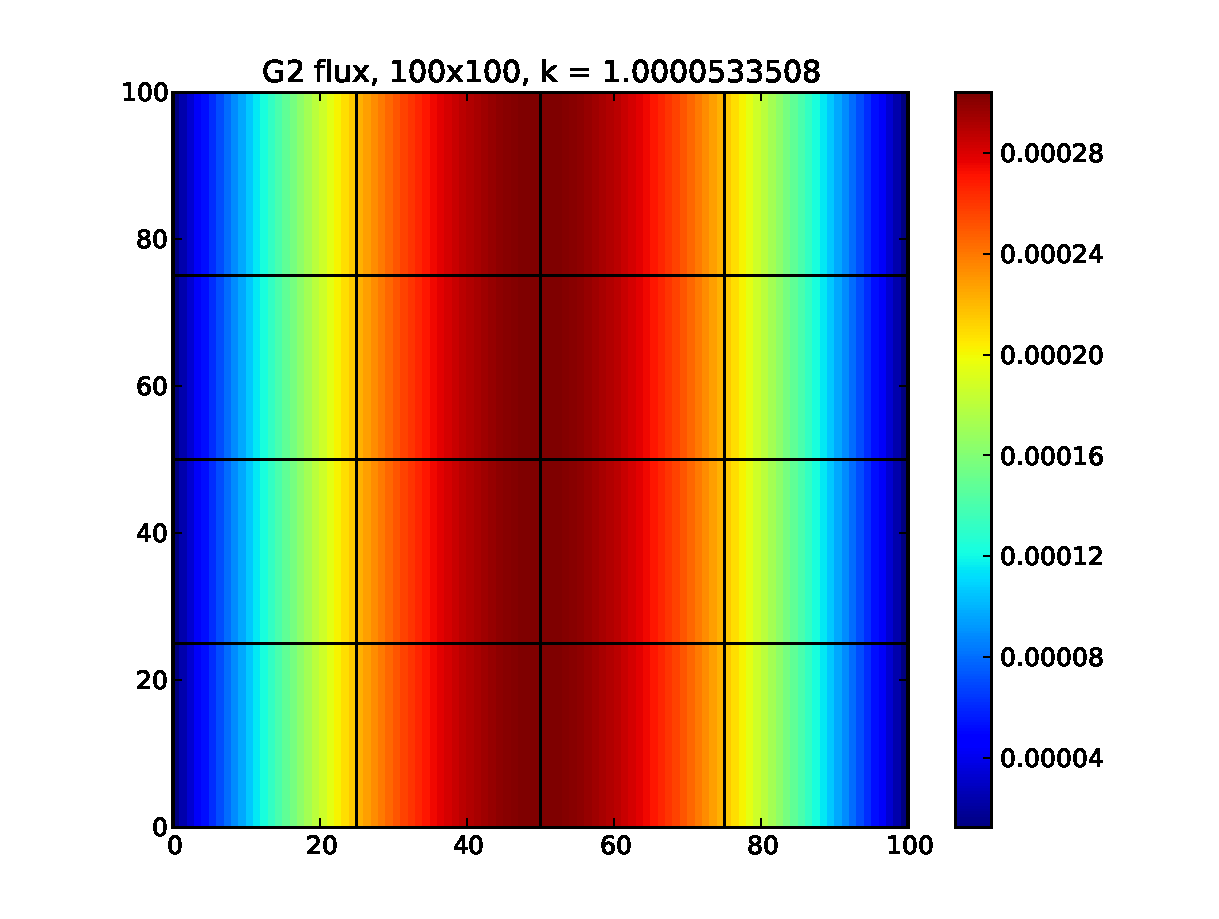
\includegraphics[width=\textwidth]{g2_50_flux}
   \caption{Low-energy flux}
  \end{subfigure}
\caption{Default Case Flux Profiles}
\label{fluxes}
\end{figure}


\section{Uniform}
We allow $\Sigma_a$ for the second energy group to vary uniformly on $\Sigma_a\in(0.08434,0.10434)$ and quantify the uncertainty using stochastic collocation for generalized polynomial expansion as well as Monte Carlo sampling.  The base case with $k$ nearly exactly one is when $\Sigma_a$ is at the mean, 0.09343.

For increasing orders of expansion, the mean and variance obtained are shown in Table \ref{runstats}.  

\begin{table}
\begin{center}
\begin{tabular}{c c|l l}
type & runs/order & mean & variance \\ \hline
MC & 1000 & 1.00373761371 & 0.00283423863458\\
SC & 2 & 1.00342873036 & 0 \\
SC & 4 & 1.00343853923 & 0.00284151047378 \\
SC & 8 & 1.00343853932 & 0.00284153558534 \\
SC & 16 & 1.00343853933 & 0.00284153558566 
\end{tabular}
\end{center}
\caption{Uniform Uncertainty Means, Variances}
\label{runstats}
\end{table}

The PDFs were obtained by Monte Carlo sampling of the polynomial expansion for the SC cases, and obtained directly for the Monte Carlo case.  Each is shown below.  The x-axis is the value of the scalar flux, and the y-axis is the probability of obtaining a particular flux.
\begin{figure}[h!]
\centering
  \begin{subfigure}[b]{0.45 \textwidth}
   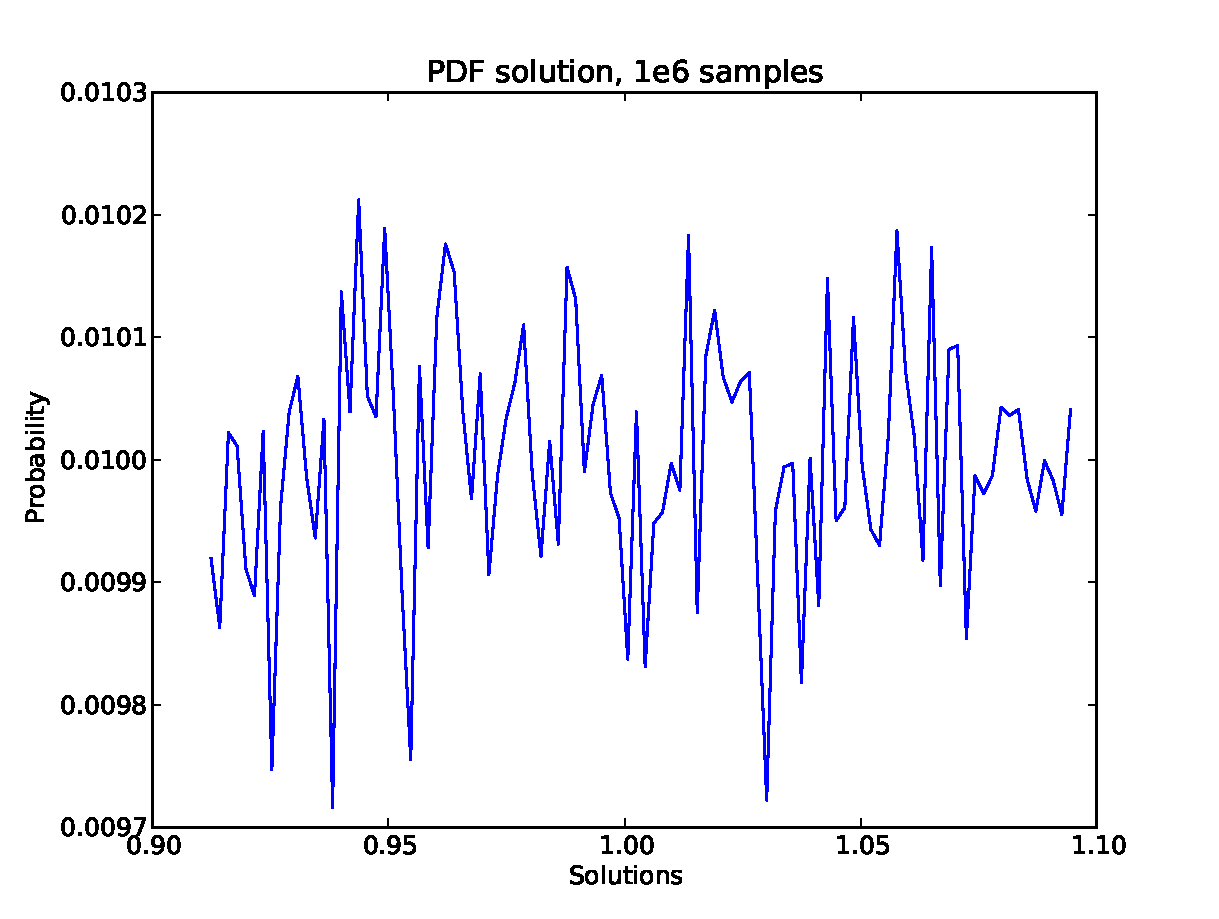
\includegraphics[width=\textwidth]{1d_sc_2_u}
   \caption{Uniform, SC order 2}
   \label{sc2}
  \end{subfigure}
  \begin{subfigure}[b]{0.45\textwidth}
   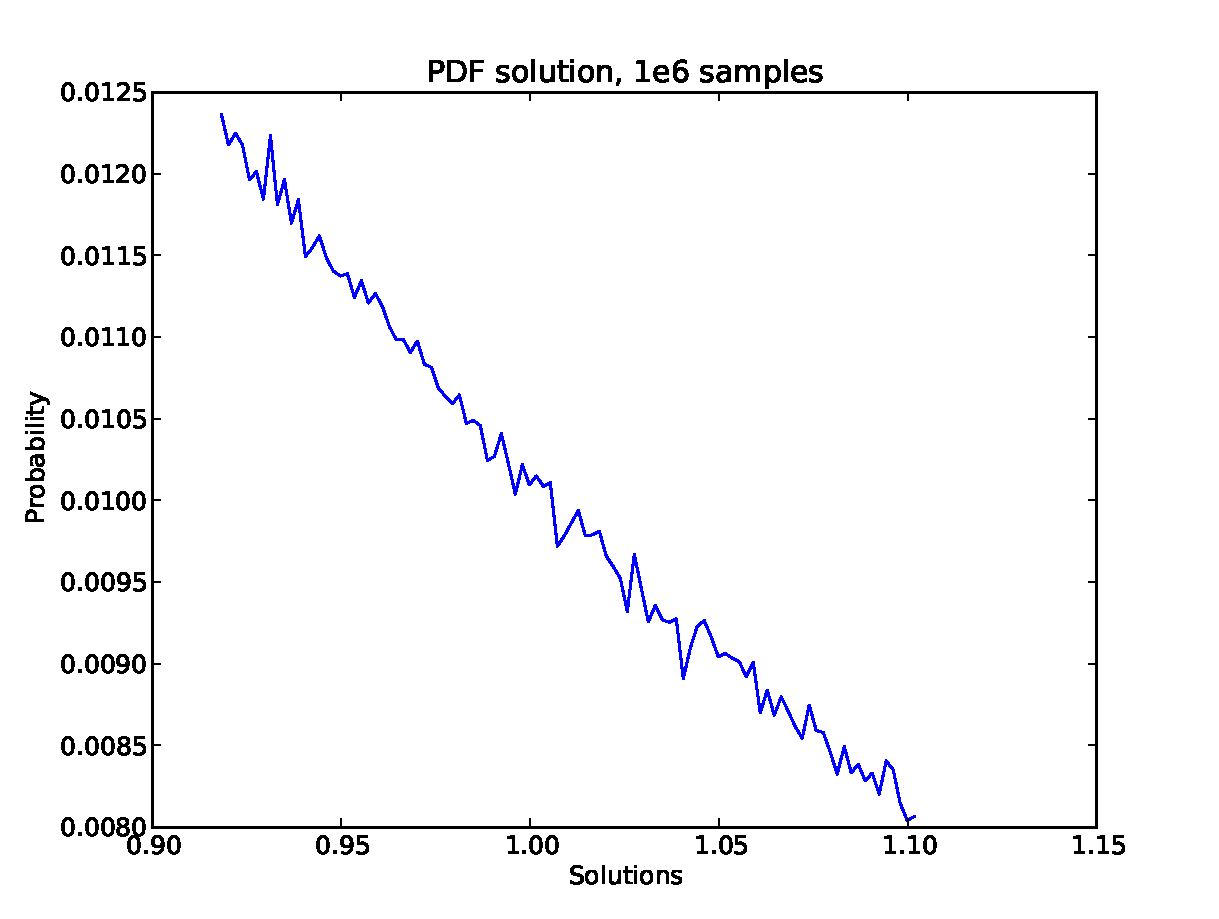
\includegraphics[width=\textwidth]{1d_sc_4_u}
   \caption{SC order 4}
   \label{Uniform, sc4}
  \end{subfigure}
\caption{Uniform, Stochastic Collocation, 2 and 4}
\end{figure}
\begin{figure}[h!]
\centering
  \begin{subfigure}[b]{0.45 \textwidth}
   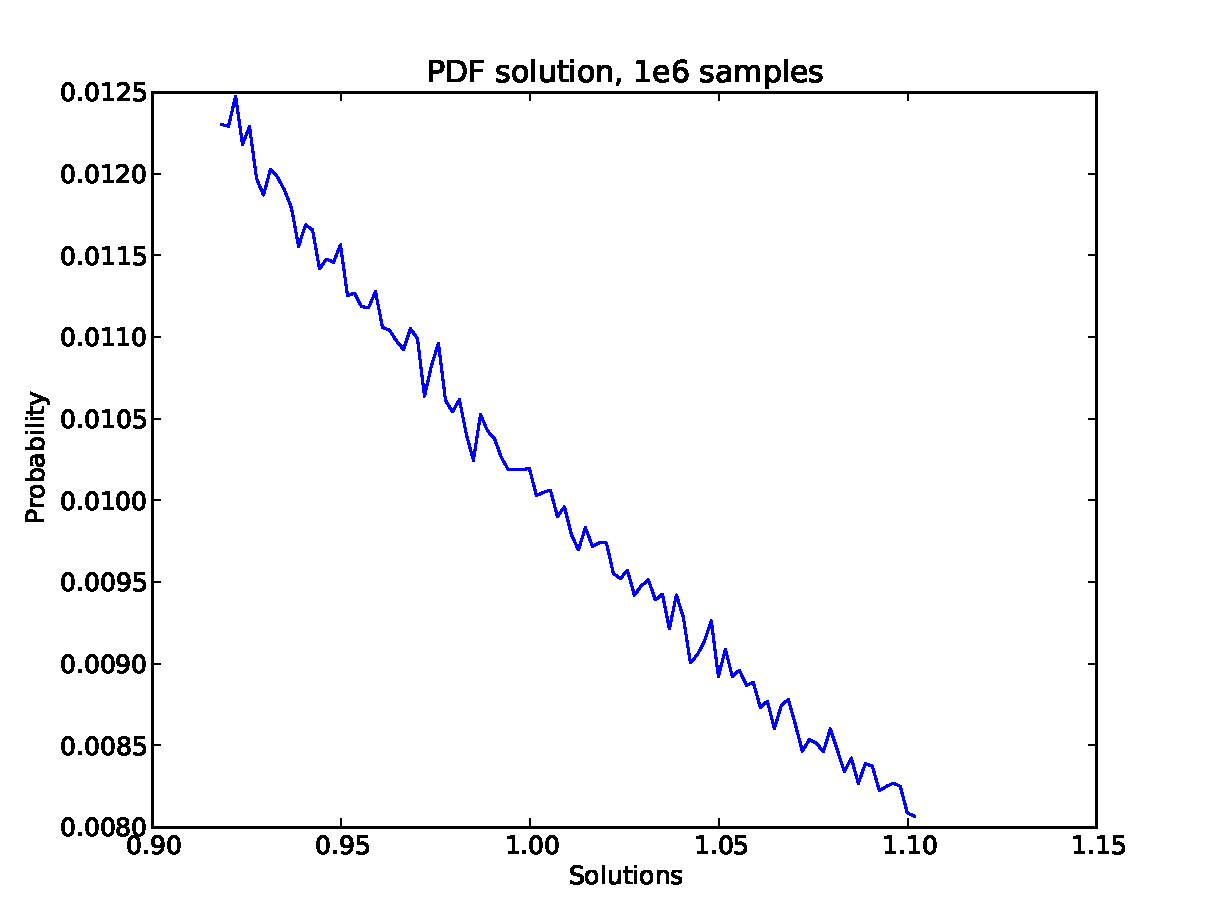
\includegraphics[width=\textwidth]{1d_sc_8_u}
   \caption{Uniform, SC order 8}
   \label{sc8}
  \end{subfigure}
  \begin{subfigure}[b]{0.45\textwidth}
   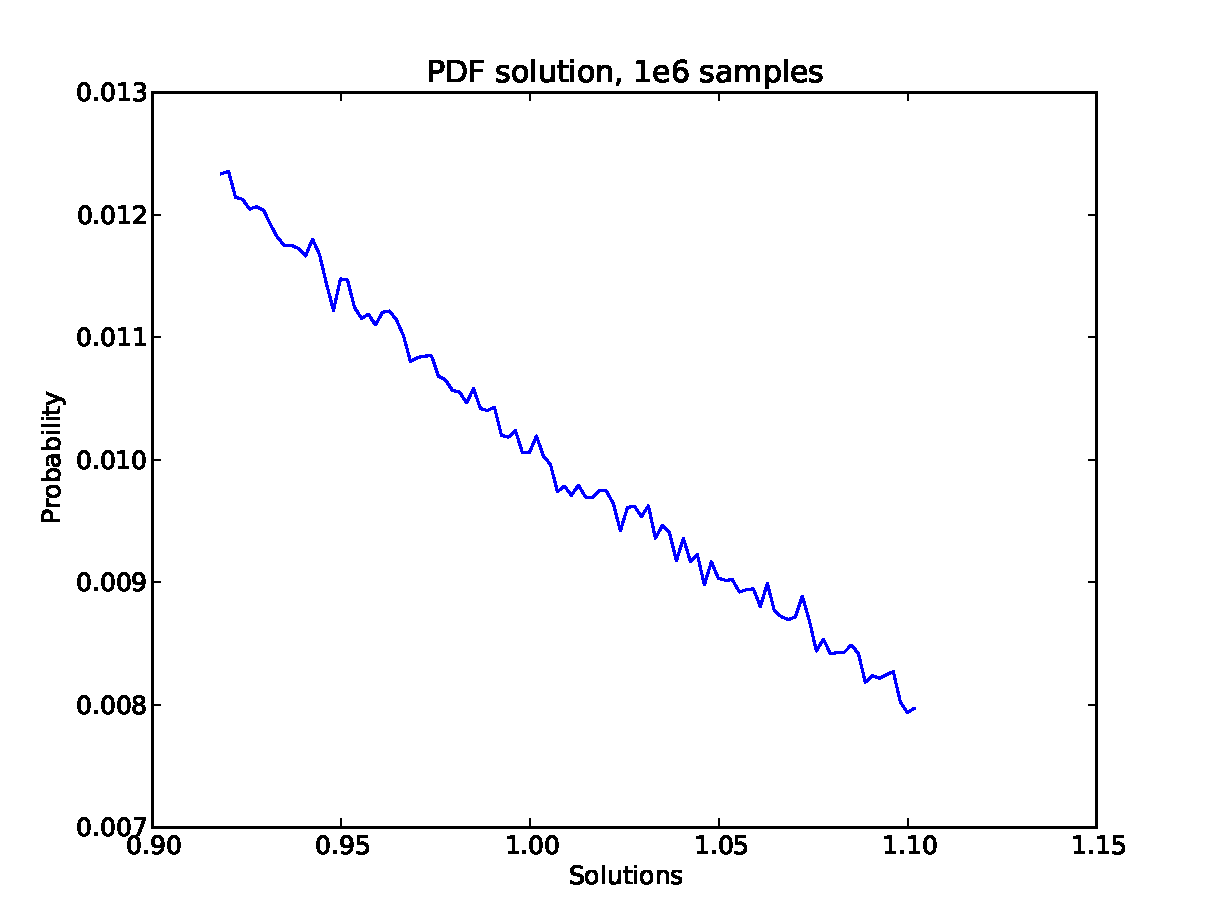
\includegraphics[width=\textwidth]{1d_sc_16_u}
   \caption{Uniform, SC order 16}
   \label{sc16}
  \end{subfigure}
\caption{Uniform, Stochastic Collocation, 8 and 16}
\end{figure}
\begin{figure}[h!]
\centering
   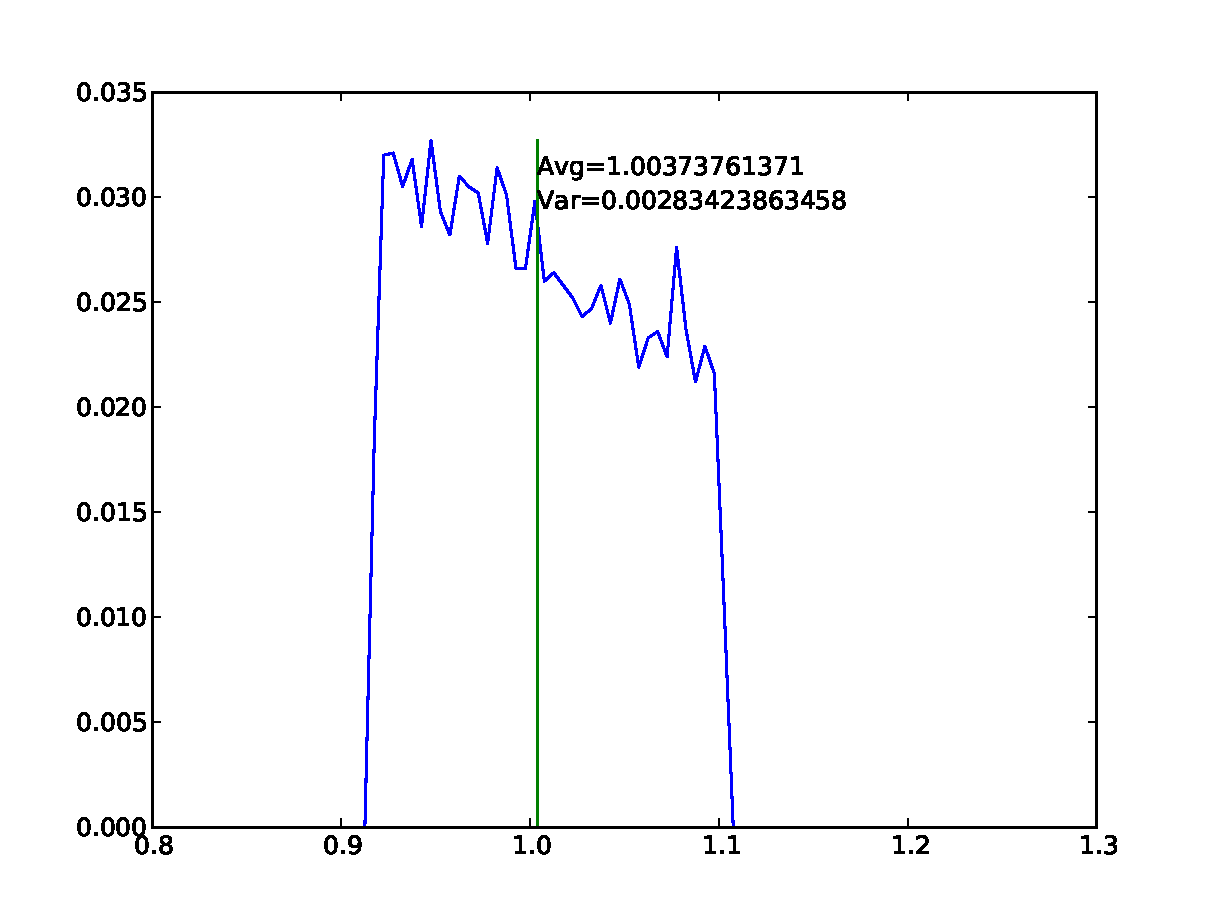
\includegraphics[width=0.5\textwidth]{1d_mc_siga_uniform_1000}
   \caption{Uniform, MC, 1000 runs }
   \label{mc}
\end{figure}


\newpage
\section{Normal}
We allow $\Sigma_a$ for the second energy group to vary normally on $\Sigma_a\in\mathcal{N}(0.09434,0.01)$ and quantify the uncertainty using stochastic collocation for generalized polynomial expansion as well as Monte Carlo sampling.

For increasing orders of expansion, the mean and variance obtained are shown along with the run time.  The other parameters for $\phi$ are taken as follows:
\begin{table}[h!]
\begin{center}
\begin{tabular}{c c|l l}
type & runs or order & mean & variance\\ \hline
MC & 1000 & 1.00846253 & 0.0068809\\
SC & 2 & 1.00999398 & 0 \\
SC & 4 & 1.01023002 & 0.00920998  \\
SC & 8 & 1.01023045 & 0.00922001 \\
SC & 16 & 1.01023045 & 0.00922001 
\end{tabular}
\end{center}
\caption{Normal Uncertainty Means, Variances}
\end{table}

The PDFs were obtained by Monte Carlo sampling of the polynomial expansion for the SC cases, and obtained directly for the Monte Carlo case.  Each is shown below.  The x-axis is the value of the scalar flux, and the y-axis is the probability of obtaining a particular flux.
\begin{figure}[h!]
\centering
  \begin{subfigure}[b]{0.45 \textwidth}
   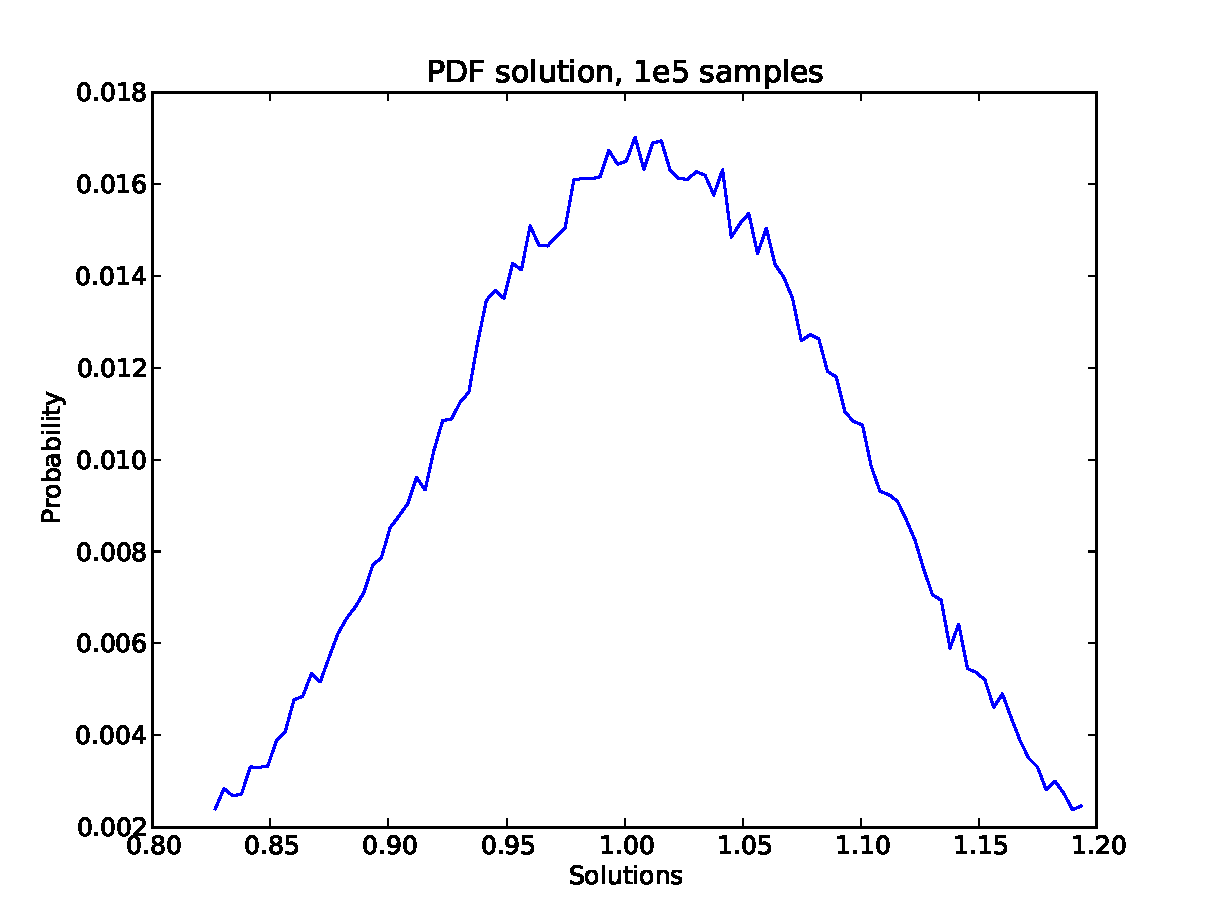
\includegraphics[width=\textwidth]{1d_sc_2_n}
   \caption{Normal, SC order 2}
   \label{sc2}
  \end{subfigure}
  \begin{subfigure}[b]{0.45\textwidth}
   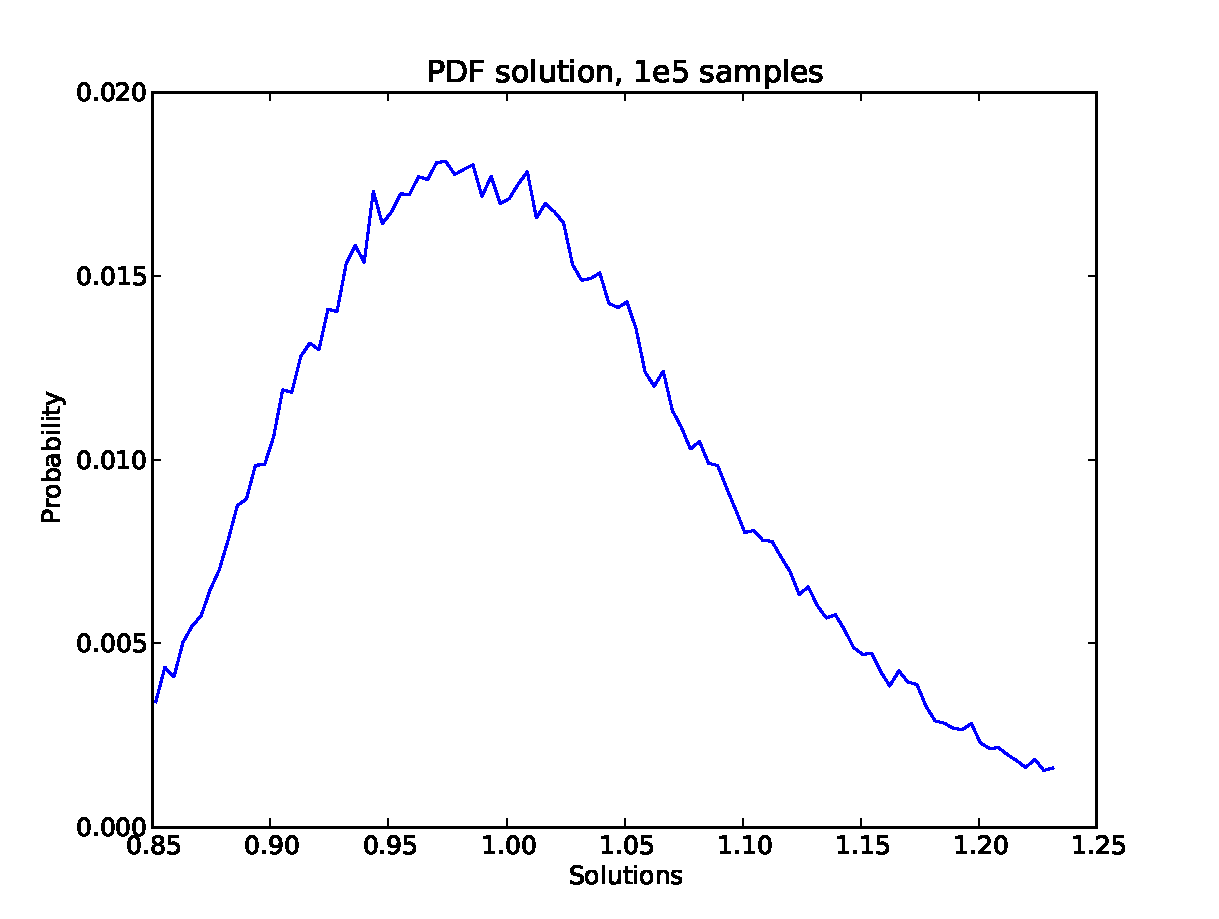
\includegraphics[width=\textwidth]{1d_sc_4_n}
   \caption{SC order 4}
   \label{Normal, sc4}
  \end{subfigure}
\caption{Normal, Stochastic Collocation, 2 and 4}
\end{figure}
\begin{figure}[h!]
\centering
  \begin{subfigure}[b]{0.45 \textwidth}
   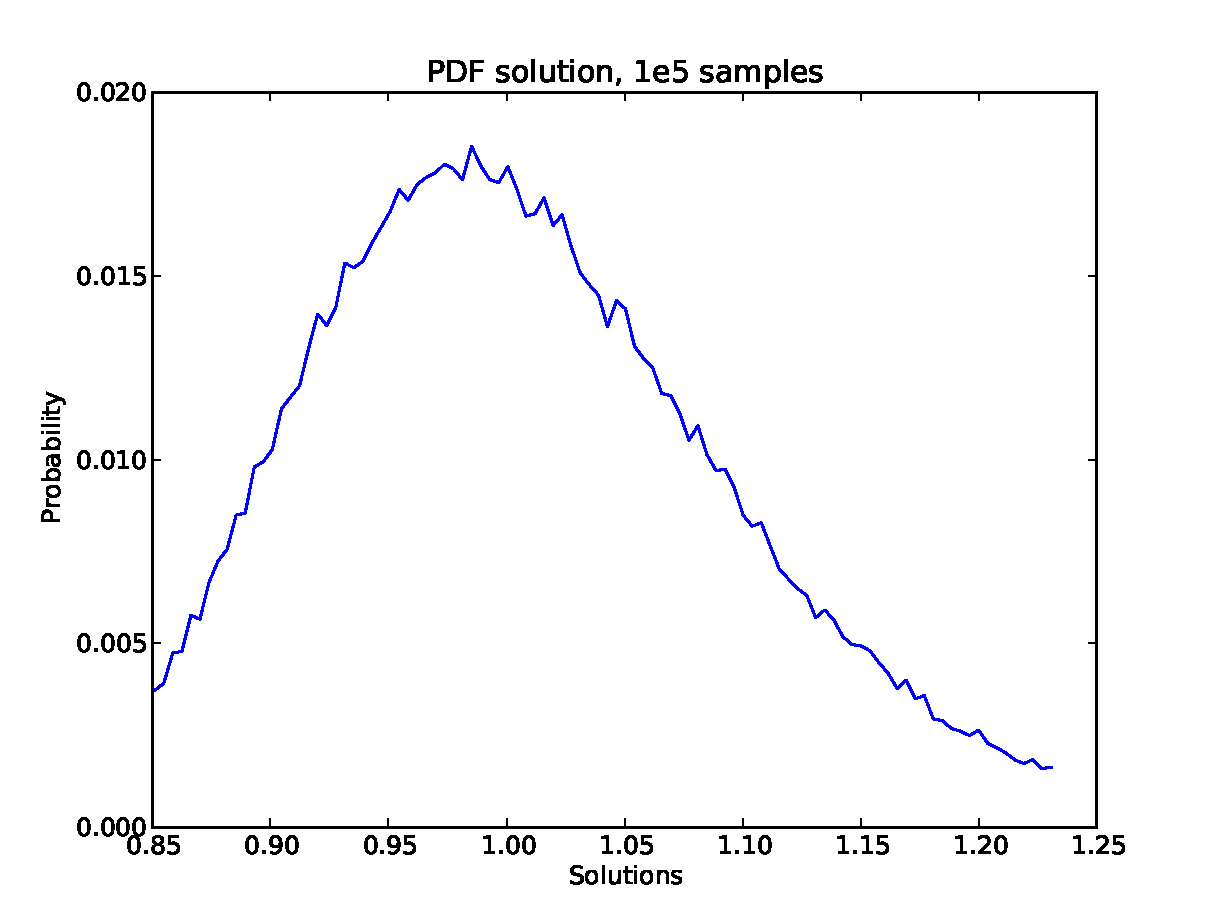
\includegraphics[width=\textwidth]{1d_sc_8_n}
   \caption{Normal, SC order 8}
   \label{sc8}
  \end{subfigure}
  \begin{subfigure}[b]{0.45\textwidth}
   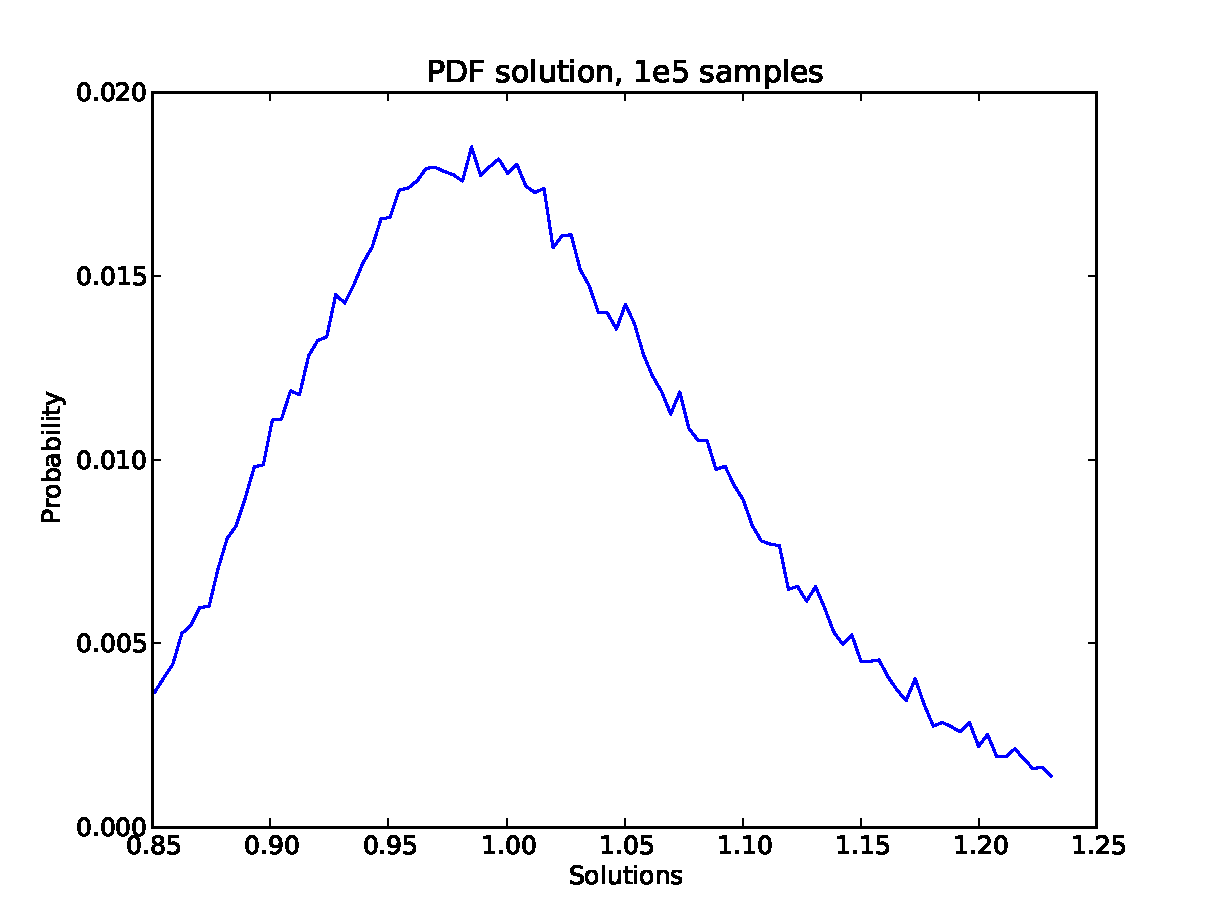
\includegraphics[width=\textwidth]{1d_sc_16_n}
   \caption{Normal, SC order 16}
   \label{sc16}
  \end{subfigure}
\caption{Normal, Stochastic Collocation, 8 and 16}
\end{figure}
\begin{figure}[h!]
\centering
   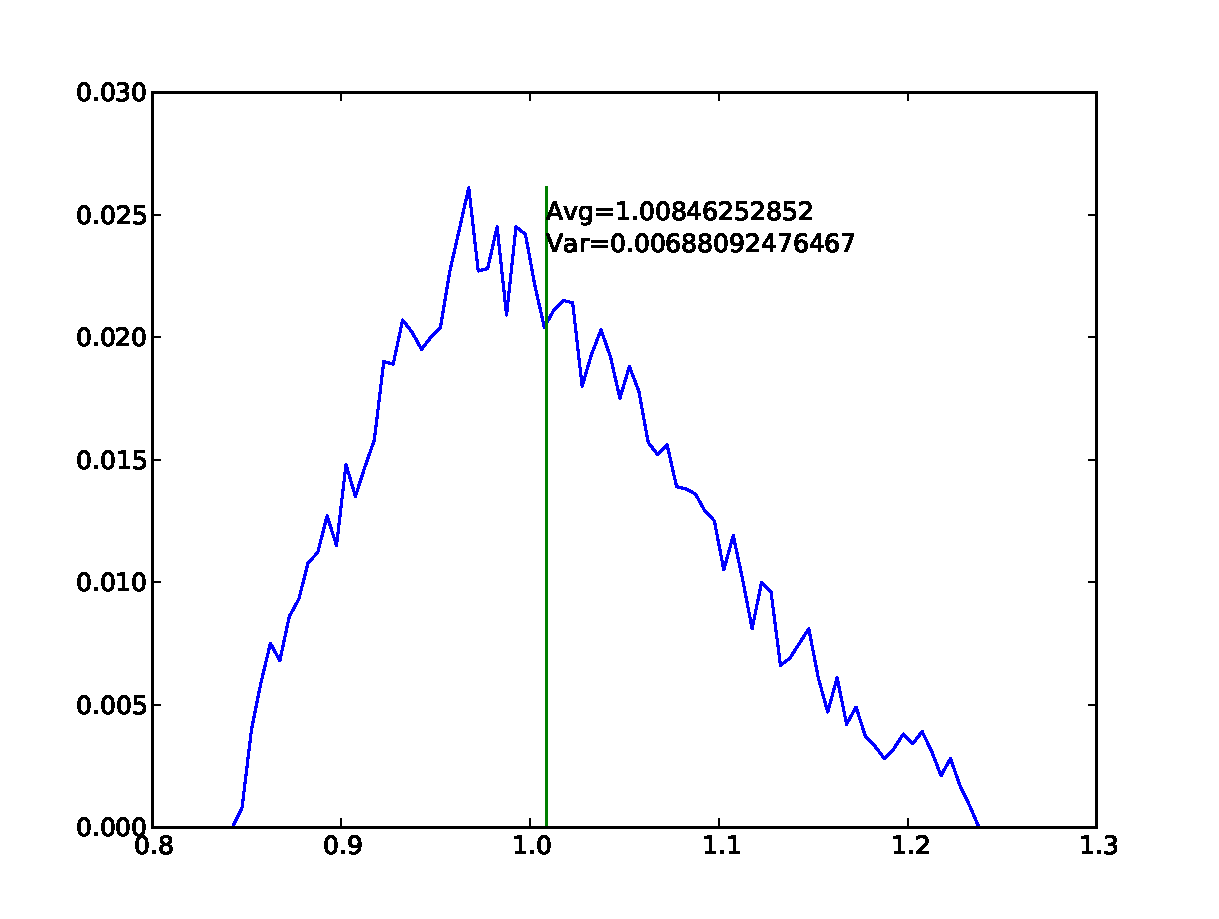
\includegraphics[width=0.5\textwidth]{1d_mc_siga_normal_1000}
   \caption{Normal, MC, 1000 runs }
   \label{mc}
\end{figure}




\end{document}


\begin{center}
\begin{tabular}{c c|c c| c}
\end{tabular}
\end{center}

\begin{figure}[h]
\centering
  \begin{subfigure}[b]{0.45 \textwidth}
   \includegraphics[width=\textwidth]{}
   \caption{}
   \label{}
  \end{subfigure}
  \begin{subfigure}[b]{0.45\textwidth}
   \includegraphics[width=\textwidth]{}
   \caption{}
   \label{}
  \end{subfigure}
\caption{}
\end{figure}